\section{Product Overview}

Cruise Activity and Service Management System là một nền tảng phần mềm mới
thay thế các quy trình quản lý rời rạc hiện tại trên du thuyền, bao gồm quản
lý lịch trình nhiều ngày, hoạt động giải trí trên tàu, tham quan bờ, đăng ký
tham gia, xác thực check-in, ghi nhận giao dịch tài khoản chi tiêu trên tàu
(onboard account) và đối soát thanh toán cuối chuyến đi.

Hệ thống được thiết kế đa nền tảng: Web Admin cho các bộ phận quản lý,
Mobile App cho hành khách, và ứng dụng Tablet/POS cho nhân viên phục vụ trực
tiếp. Do đặc thù kết nối mạng trên tàu không ổn định, hệ thống hỗ trợ ghi
nhận giao dịch ngoại tuyến và tự động đồng bộ dữ liệu khi có kết nối trở lại.

Sơ đồ ngữ cảnh bên dưới minh họa các thực thể bên ngoài (external entities)
và giao diện hệ thống cho phiên bản phát hành 1.0. Hệ thống dự kiến sẽ mở
rộng ở các phiên bản sau, bổ sung tự động hóa nâng cao và tích hợp thêm các
nền tảng thanh toán/vận hành khác.

\begin{figure}[H]
    \centering
    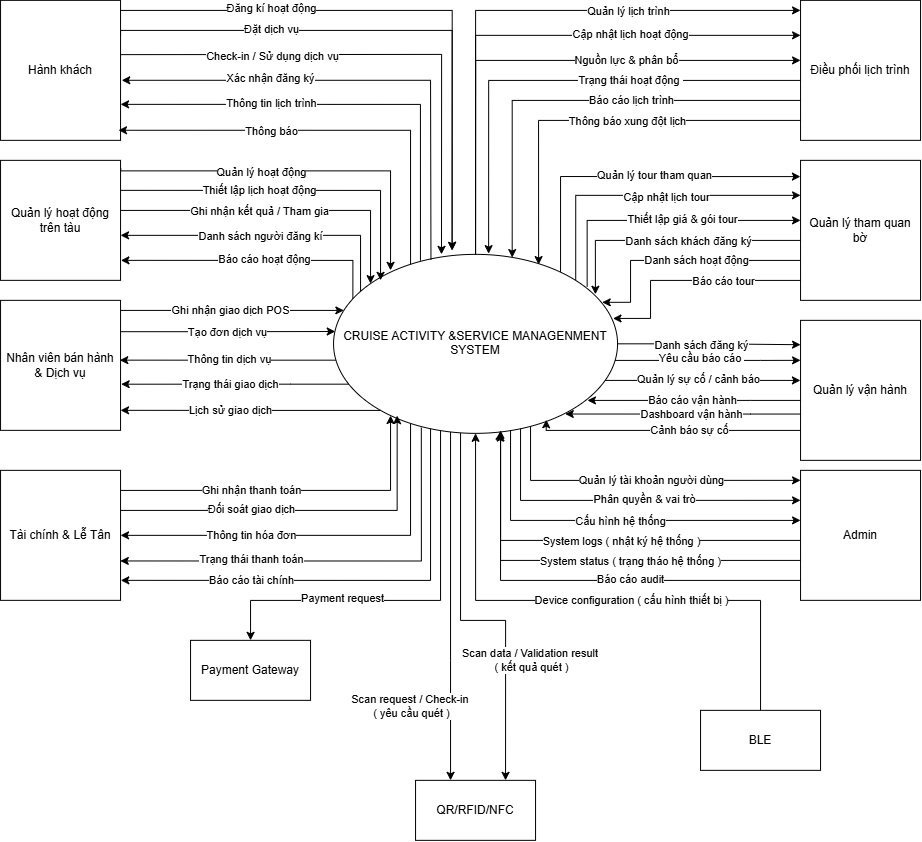
\includegraphics[width=0.82\textwidth]{images/system-context-diagram.png}
    \caption{Sơ đồ ngữ cảnh hệ thống (System Context Diagram)}
    \label{fig:context-diagram}
\end{figure}

\subsection{Mô tả luồng dữ liệu và ràng buộc nghiệp vụ}

Hệ thống hoạt động theo mô hình offline-first: mọi giao dịch, check-in, đăng ký
và lịch trình quan trọng đều được lưu tạm trên thiết bị cục bộ trước khi giao
cho các dịch vụ trung tâm. Khi có kết nối mạng, hệ thống tiến hành đồng bộ dữ
liệu theo quy trình xác thực, kiểm tra trùng lặp và cập nhật trạng thái cuối
cùng. Mô hình này giúp cải thiện độ tin cậy ở các tuyến đường có tín hiệu yếu
hoặc không ổn định trong quá trình tàu di chuyển.

\begin{longtable}{|p{2.8cm}|p{3.2cm}|p{7.2cm}|}
    \hline
    \textbf{Mô đun} & \textbf{Vai trò} & \textbf{Mô tả trách nhiệm} \\ \hline
    \endfirsthead
    \hline
    \textbf{Mô đun} & \textbf{Vai trò} & \textbf{Mô tả trách nhiệm} \\ \hline
    \endhead
    Client Web Admin & Quản trị & Cài đặt cấu hình hệ thống, quản lý quyền, giám sát hoạt động và doanh thu \\ \hline
    Mobile App & Hành khách & Xem lịch trình, đăng ký hoạt động, check-in, xem chi phí và nhận thông báo \\ \hline
    Tablet/POS & Nhân viên & Đăng nhập nhanh, quét QR/RFID/NFC, ghi nhận giao dịch và xác thực thanh toán \\ \hline
    API Gateway & Truyền tải & Tiếp nhận, định tuyến và kiểm soát truy cập cho mọi API trong hệ thống \\ \hline
    Business Service & Logic nghiệp vụ & Xử lý đăng ký, lịch trình, khuyến nghị và business rules \\ \hline
    Sync Engine & Đồng bộ & Đồng bộ dữ liệu ngoại tuyến, giải quyết xung đột và tái tạo trạng thái \\ \hline
    Reporting Service & Báo cáo & Tạo báo cáo vận hành, tài chính và thống kê theo chuyến đi \\ \hline
    \caption{Bảng phân tích thành phần hệ thống theo mô đun chức năng}
\end{longtable}
\FloatBarrier
